\section{Implementierung der OPA}
In diesem Abschnitt geht es um eine Implementierung einer Bibliothek für OPA in einer Programmiersprache. Dazu folgt eine kurze Aufzählung der verwendeten Programme und Ressourcen und anschließend folgt eine Erläuterung zu der Funktionsweise anhand eines Klassendiagramms.
\paragraph*{Verwendete Ressourcen}
Die Bibliothek wurde in der Programmiersprache Java mit dem JDK 1.8 verfasst. Die Sprache Java ist sehr weit verbeitet und sehr gut dokumentiert und vereinfacht strukturiertes und methodisches Vorgehen. Als Umwickelungsumgebung wurde IntelliJ IDEA Ultimate Edition verwendet. Für die Erstellung der Bibliothek  als JAR-Datei und die Verwaltung der Abhängigkeien wurde das Werkzeug Maven der Apache Software Foundation verwendet. Außer den Standardbibliotheken der JDK 1.8 wurde noch \textit{java-tuples} verwendet.

\paragraph*{Design}
Für die Entwickelung wurde hauptsächlich die Definition des OPA direkt in Klassen und Attribute umgesetzt. So besteht zB. die Klasse \textit{OP\_Automat} aus einer Menge von Terminalen (Character), einer OP\_Matrix, einer Menge von Zuständen, der Menge der Start- und Endzustände und einem Objekt der \textit{Transitionen-}Klasse, was der Übergangsfunktion $\delta$ entspricht. Die Präzedenzrelation werden als Enumeration dargestellt. In \autoref{uml1} ist ein vereinfachtes Klassendiagramm für das Paket model.automation dargestellt. 
\begin{figure}
\centering
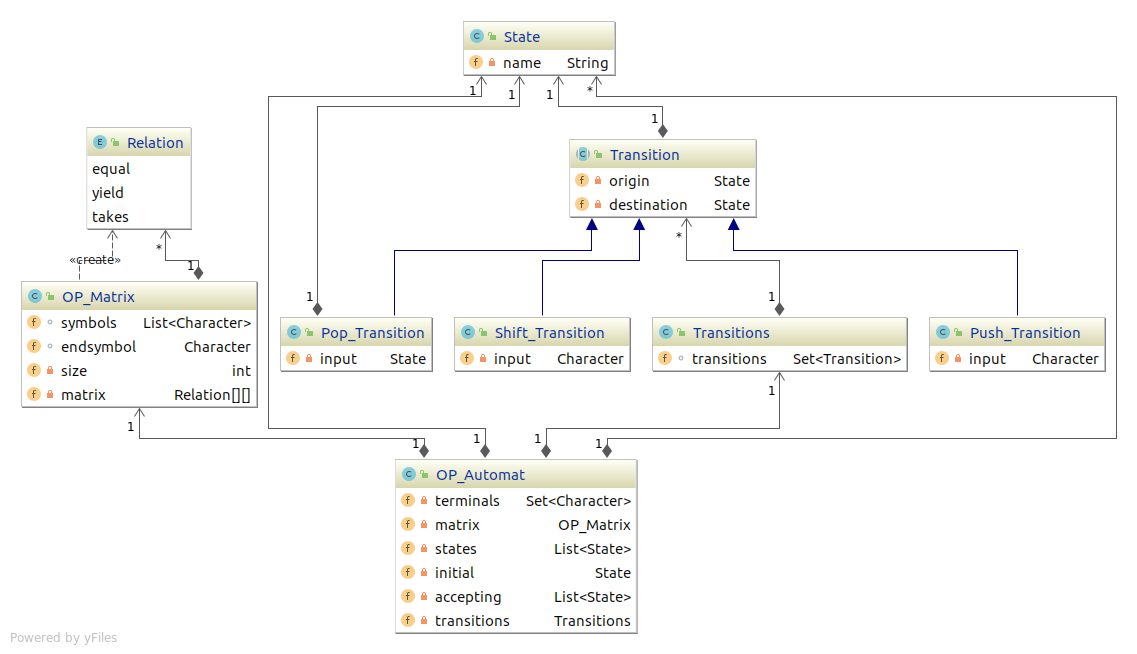
\includegraphics[scale=0.3]{sections/automaton}
\caption{UML Klassendiagramm zum automaton package}
\label{uml1}
\end{figure}
 Wie in den Quellen ist auch hier die Berechnung erst einmal vom reinen Automatenmodell getrennt. Die Berechnung findet in den Klassen des Paketes model.computation statt, welches wie in \autoref{uml2} beschrieben aufgebaut ist. 
 \begin{figure}
 \centering
 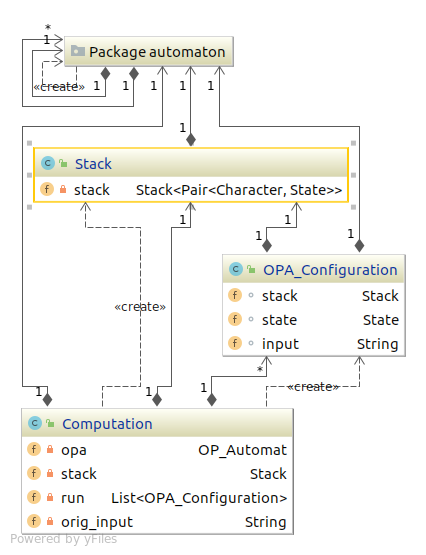
\includegraphics[scale=0.35]{sections/computation}
 \caption{UML Klassendiagramm zum computation package}
 \end{figure}
Um nun eine Berechnung zu starten muss nunächst der Automat initialisiert werden. Dieser besteht aus vielen verschachtelten Attributen, was die Initialisierung sehr aufwendig macht. Es wurde unter anderem durch Verwendung des Builder-Patterns für den Automaten und einer ähnlichen Form für die Matrix und die Transitionen eine etwas komfortablere und intuitivere Nutzung gewährleistet. Dann muss ein Objekt der Klasse \textit{Computation} mit einem OPA und einem Eingabestring erzeugt werden, welches dann durch die \textit{compute} Methode die Berechnung startet und das Ergebnis in der Konsole ausgibt. Um schnelleres Testen zu gewährleisten, wurde ebenfalls eine OPA\_ReaderWriter Klasse erzeugt, die es ermöglicht den Automaten zu serialisieren und somit zu speichern. Das entstandene Format ist dabei allerdings nicht leserlich. Weiterhin wurden zu allen wichtigen Komponenten \textit{print-} Methoden implementiert.\\
Der Automat arbeitet nichtdeterministisch, indem er in jedem Schritt alle möglichen weiteren Schritte berechnet. Am Anfang wird zu jedem initialen Zustand eine Konfiguration erstellt. Es wird immer nur ein Pfad von Konfigurationen bearbeitet bis dieser akzeptiert oder fehlschlägt. An jeder Stelle werden mögliche Alternativen in einer zweiten Warteschlange gespeichert, mit der Information an welcher Stelle diese Alternative einzusetzen ist. Schlägt ein Pfad fehl, wird der Lauf bis zur jüngsten Alternative in der Warteschlange zurückgesetzt und es geht mit der Alternative weiter. Wenn eine akzeptierende Konfiguration erreicht wird, oder keine Alternativen mehr vorhanden sind bei nichtleerem Input, terminiert der Automat. \\
Die Implementierung ist allerdings noch sehr rudimentär und es konnten leider nicht alle Anforderungen erfüllt werden. Es wäre schön gewesen, Konstruktionen für die Abschlusseigenschaften auf Automatenebene zu haben, so konnte lediglich die Vereinigung implementiert werden.